\ifx\allfiles\undefined
\documentclass[12pt, a4paper, oneside, UTF8]{ctexbook}
\def\path{../config}
\usepackage{amsmath}
\usepackage{amsthm}
\usepackage{amssymb}
\usepackage{graphicx}
\usepackage{mathrsfs}
\usepackage{mathtools}
\usepackage{pifont}  % 多种符号
\usepackage{enumitem}
\usepackage{geometry}
\usepackage[colorlinks, linkcolor=black]{hyperref}
\usepackage{stackengine}
\usepackage{yhmath}
\usepackage{extarrows}
\usepackage{unicode-math}
\usepackage{caption}
\usepackage{ulem}  % 各种标记线
\usepackage{xargs}  % 多缺省命令
\usepackage{bm}  %  加粗数学字符 

\usepackage{fancyhdr}
\usepackage[dvipsnames, svgnames]{xcolor}
\usepackage{listings}
\usepackage{zhlipsum}  % 随机中文文本, 测试用
\usepackage{lipsum}  % 随机英文文本, 测试用

\definecolor{mygreen}{rgb}{0,0.6,0}
\definecolor{mygray}{rgb}{0.5,0.5,0.5}
\definecolor{mymauve}{rgb}{0.58,0,0.82}

\graphicspath{{figure/}, {../figure/}, {config/}, {../config/}}

% 设置图标签格式
\captionsetup[figure]{
    labelfont={bf},labelformat={default},labelsep=period,name={Fig.}}

\linespread{1.6}

\geometry{
    top=25.4mm, 
    bottom=25.4mm, 
    left=20mm, 
    right=20mm, 
    headheight=2.17cm, 
    headsep=4mm, 
    footskip=12mm
}

\setenumerate[1]{itemsep=5pt, partopsep=0pt, parsep=\parskip, topsep=5pt}
\setitemize[1]{itemsep=5pt, partopsep=0pt, parsep=\parskip, topsep=5pt}
\setdescription{itemsep=5pt, partopsep=0pt, parsep=\parskip, topsep=5pt}

\lstset{
    language=Mathematica,
    basicstyle=\tt,
    breaklines=true,
    keywordstyle=\bfseries\color{NavyBlue}, 
    emphstyle=\bfseries\color{Rhodamine},
    commentstyle=\itshape\color{black!50!white}, 
    stringstyle=\bfseries\color{PineGreen!90!black},
    columns=flexible,
    numbers=left,
    numberstyle=\footnotesize,
    frame=tb,
    breakatwhitespace=false,
} 


\usepackage{tcolorbox}

\tcbuselibrary{most}

% 定义单独编号,其他四个共用一个编号计数 (原版),这里只列举了五种,其他可类似定义(未定义的使用原来的也可)
\newtcbtheorem[number within=section]{defn}
    {定义}{colback=Salmon!20, colframe=Salmon!90!Black, fonttitle=\bfseries}{def}

\newtcbtheorem[number within=section]{lemma}
    {引理}{colback=OliveGreen!10, colframe=Green!70, fonttitle=\bfseries}{lem}

% 使用另一个计数器可加参数 use counter from=lemma
\newtcbtheorem[number within=section]{them}
    {定理}{colback=SeaGreen!10!CornflowerBlue!10, 
           colframe=RoyalPurple!55!Aquamarine!100!,
           fonttitle=\bfseries}{them}

\newtcbtheorem[number within=section]{criterion}
    {准则}{colback=green!5, colframe=green!35!black, fonttitle=\bfseries}{cri}

\newtcbtheorem[number within=section]{corollary}
    {推论}{colback=Emerald!10, colframe=cyan!40!black, fonttitle=\bfseries}{cor}

\newtcbtheorem[number within=section]{proposition}
    {命题}{colback=red!5,colframe=red!75!black,fonttitle=\bfseries}{prop}
% red!5,colframe=red!75!black 警告框
% 使用格式是\begin{***}{}{} \end{***} ,需要两个 {}{} ,可以不填,但要有.
% 第一个 {} 填入别名 第二个为引用的 label
% 引用方法为 \ref{def:xxx}

\newtheorem{example}{\indent \color{SeaGreen}{例}}[section]
\theoremstyle{plain}
\newtheorem*{rmk}{\indent 注}
\renewenvironment{proof}{\indent\textcolor{SkyBlue}{\textbf{证明:}}\;}{\qed\par}
\newenvironment{solution}{\indent\textcolor{SkyBlue}{\textbf{解:}}\;}{\qed\par}
% \def\d{\mathrm{d}}
\def\R{\mathbb{R}}
\newcommand\mi{\mathrm{i}} 
\newcommand\me{\mathrm{e}}
\newcommand*{\dif}{\mathop{}\!\mathrm{d}}  % 微分算符 d
% \newcommand{\bs}[1]{\boldsymbol{#1}}
\newcommand{\ora}[1]{\overrightarrow{#1}}
\newcommand{\myspace}[1]{\par\vspace{#1\baselineskip}}
\newcommand{\xrowht}[2][0]{\addstackgap[.5\dimexpr#2\relax]{\vphantom{#1}}}
\newenvironment{ca}[1][1]{\linespread{#1} \selectfont \begin{cases}}{\end{cases}}
\newenvironment{vx}[1][1]{\linespread{#1} \selectfont \begin{vmatrix}}{\end{vmatrix}}
\newcommand{\tabincell}[2]{\begin{tabular}{@{}#1@{}}#2\end{tabular}}
\newcommand{\pll}{\kern 0.56em/\kern -0.8em /\kern 0.56em}
\newcommand{\bit}[1]{\symbfit{#1}}  % 加粗斜体
\newcommand{\Div}[1]{\mathrm{div}\;#1}  % 散度 div
\newcommand{\grad}[1]{\mathrm{grad}\;#1}  % 梯度 grad
\newcommand{\Rot}[1]{\mathrm{rot}\;#1}  % 旋度 rot
\newcommand*{\colorstar}[1][black]{\textcolor{#1}{\ast\quad}}  % 星星开头的重点行 (可改变星星颜色)
% 彩色的文字及下划线
\newcommandx*{\coloruline}[3][1=black, 2=black, usedefault]{
    \textcolor{#1}{\!\uline{\textcolor{#2}{#3}}}}  % 未完成此功能,下划线换行问题

\def\myIndex{0}  % 封面
% \input{\path/cover_package_\myIndex.tex}

\def\myTitle{数学物理方程}
\def\myAuthor{高峰}
\def\myDateCover{2020 年 12 月 16 日\ --}
\def\myDateForeword{\today}
\def\myForeword{前言}
\def\myForewordText{
    
}
\def\mySubheading{}


\begin{document}
% \input{\path/cover_text_\myIndex.tex}

\newpage
\thispagestyle{empty}
\begin{center}
    \Huge\textbf{\myForeword}
\end{center}
\myForewordText
\begin{flushright}
    \begin{tabular}{c}
        \myDateForeword
    \end{tabular}
\end{flushright}

\newpage
\pagestyle{plain}
\setcounter{page}{1}
\pagenumbering{Roman}
\tableofcontents

\newpage
\pagenumbering{arabic}
\setcounter{chapter}{0}  % 从第一章开始计数
\setcounter{page}{1}

\pagestyle{fancy}
\fancyfoot[C]{\thepage}
\renewcommand{\headrulewidth}{0.4pt}
\renewcommand{\footrulewidth}{0pt}








\else
\fi

\chapter{数学物理定解问题}

\section{基本概念}

方程:含有未知量的等式。(\hyperref[fig:方程分类]{Fig.~\ref{fig:方程分类}})

\begin{figure}
    \centering
    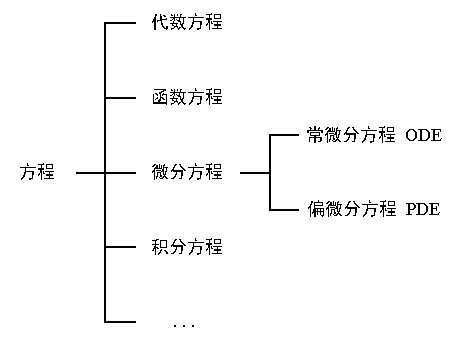
\includegraphics{方程分类.pdf} 
    \caption{\label{fig:方程分类} 方程分类}
\end{figure}
\begin{defn}{偏微分函数}{}
    关于多元函数 $ u(x,y,\cdots) $ 及其某些偏导数的关系式:
    \[ 
        F(x, y, \cdots, u, u_x, u_y, \cdots, u_{xx}, u_{xy}, u_{yy}, \cdots, 
        u_{xxx}, u_{xxy},\cdots) = 0, 
    \]
    其中 $F$ 是 $x$, $y$, $\cdots$, $u$ 及 $u$ 的有限多个偏导数的已知函数。
\end{defn}
\begin{rmk}{}
    偏微分方程(1)未知函数是多元函数,且未知数个数有限;
    (2)包含未知函数的某些偏导数的方程。
\end{rmk}

偏微分方程的研究集中在少数特殊类型的偏微分方程,一般性较少,个性多。

偏微分方程的解  \\
\textcolor{red}{偏微分方程的通解是含有自变量的任意函数}

偏微分方程的阶
% TODO: 使用红色下划线
\noindent 线性偏微分方程(\hyperref[fig:偏微分方程分类]{Fig.~\ref{fig:偏微分方程分类}})
:方程中实际所含未知数的各阶偏导数是线性的。  \\
自由项:在\textcolor{red}{线性偏微分方程}中,不含 $u$ 及它的偏导数的项。  \\
线性方程中,自由项为 0 的是齐次偏微分方程,自由项不为 0 的是非齐次偏微分方程。  \\
线性方程的叠加原理  \\
非线性偏微分方程:不是线性的统称非线性。  \\
拟线性偏微分方程:在非线性偏微分方程中,关于未知函数的所有最高阶偏导数都是线性的。  \\
主部:在拟线性偏微分方程中,由最高阶偏导数组成的部分。  \\
半线性:主部的系数都是常数或是自变量的已知函数。  \\
完全非线性偏微分方程:既不是线性,也不是拟线性的偏微分方程。

\begin{figure}
    \centering
    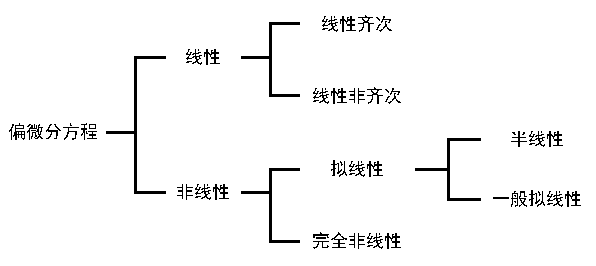
\includegraphics{偏微分方程分类.pdf}
    \caption{\label{fig:偏微分方程分类} 偏微分方程分类}
\end{figure}

\section{二阶偏微分方程}

二阶 PDE 的分类 (\hyperref[fig:二阶PDE]{Fig.~\ref{fig:二阶PDE}})  \\
二阶线性 PDE 的判别式 $ \Delta = a_{12}^2-a_{11}a_{22} 
    \begin{cases} > 0 & \mbox{双曲型}  \\  
        = 0 & \mbox{抛物型}  \\
        < 0 & \mbox{椭圆型}
    \end{cases} $  \\
二阶线性 PDE 的特征方程:
\[ a_{11}(\frac{\dif y}{\dif x})^2 - 2a_{12}\frac{\dif y}{\dif x} + a_{22} = 0\]
\colorstar 二阶 PDE 化简的一个方法  \\
原方程为 $a_{11}u_{xx} + 2a_{12}u_{xy} + a_{22}u_{yy}
    + b_1u_x + b_2u_y + cu = f$,则:
\[ \begin{bmatrix}
        \overline{a_{11}} & \overline{a_{12}}  \\
        \overline{a_{21}} & \overline{a_{22}}
    \end{bmatrix} = \bit{Q} 
    \begin{bmatrix}
        a_{11} & a_{12}  \\
        a_{21} & a_{22}
    \end{bmatrix} \bit{Q}^T,\ \mbox{其中}\ \bit{Q} = 
    \begin{bmatrix}
        \xi_{x} & \xi_{y}  \\
        \eta_{x} & \eta_{y}
    \end{bmatrix},\]
\[ \overline{b_{1}} = (L - c)\xi,\quad \overline{b_{2}} = (L - c)\eta,\quad
    \overline{c} = c,\quad \overline{f} = f,\]
其中 $ L = a_{11}\frac{\partial ^{2}}{\partial ^{2} x^{2}}
    + 2a_{12}\frac{\partial ^{2}}{{\partial {x}}{\partial {y}}}
    + a_{22}\frac{\partial ^{2}}{\partial ^{2} y^{2}} 
    + b_{1}\frac{\partial}{\partial x}
    + b_{2}\frac{\partial}{\partial y} + c,$
$\overline{b_{1}}$ 等为新方程的对应参数。

\begin{figure}
    \centering
    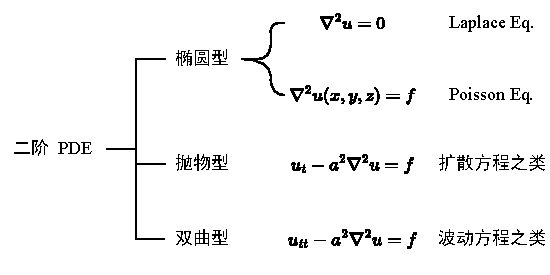
\includegraphics{二阶PDE.pdf}
    \caption{\label{fig:二阶PDE} 二阶PDE}
\end{figure}

\noindent \colorstar 拉普拉斯 Laplace 算符:

一维 $\Delta_1 = \nabla\cdot\nabla
    = \frac{\partial ^{2}}{\partial ^{2} x^{2}}$
    
二维 $\Delta_2 = \nabla\cdot\nabla
    = \frac{\partial ^{2}}{\partial ^{2} x^{2}}
    + \frac{\partial ^{2}}{\partial ^{2} y^{2}}$
    
三维 $\Delta_3 = \nabla\cdot\nabla = \nabla^2 
    = \frac{\partial ^{2}}{\partial ^{2} x^{2}}
    + \frac{\partial ^{2}}{\partial ^{2} y^{2}}
    + \frac{\partial ^{2}}{\partial ^{2} z^{2}}$
    
四维 $\Delta_4 = \square\cdot\square
    = \frac{\partial ^{2}}{\partial ^{2} x^{2}}
    + \frac{\partial ^{2}}{\partial ^{2} y^{2}}
    + \frac{\partial ^{2}}{\partial ^{2} z^{2}}
    - \frac{1}{c^2}\frac{\partial ^{2}}{\partial ^{2} t^{2}}$。

(\textcolor{blue}{四维的 Laplace 算符就是达朗贝尔算符})

\section{定解问题}

\begin{equation*}
    \mbox{泛定方程} + \mbox{定解条件}
        \left\{ 
            \begin{lgathered} \mbox{初始条件} \\ \mbox{边界条件} \end{lgathered}   
        \right.
    = \mbox{定解问题}
        \left\{
            \begin{lgathered} 
                \mbox{初值问题(也叫做 Cauthy 问题)} \\ \mbox{边值问题} \\ \mbox{混合问题} 
            \end{lgathered} 
        \right.
\end{equation*}
泛定方程(\textcolor{red}{描绘普遍规律的方程});
Cauthy 问题(\textcolor{blue}{只有初始条件,没有(无需)边界条件});
\textcolor{blue}{条件可以为分段函数}。 \\
\colorstar $\mbox{对时间求导的阶数} = \mbox{所需的初始条件个数} $

守恒律:对任意的 $Q$,$Q$ 内的该物质的变化率 $=$ 净流入 $+$ $Q$内的总生成率

\noindent 例如:$u_t = -\;\Div{\bit{\Phi}} + f(x, t, u)$。  \\  % TODO div 前空格
守恒律是对各种物理过程普适的方程(共性)。
\[ \mbox{偏微分方程} = \mbox{守恒律} + \mbox{本构关系(特性定律)} \]

适定性:(1)存在性;(2)唯一性;(3)稳定性。

\noindent 三类典型的边界条件(以热传导方程为例)  \\
(1) 第一边值问题或狄利克雷问题  \\
边界条件:
 \[ u|_\varGamma = \varphi(x,y,z,t),\quad \varphi\ \mbox{为定义在}\ (x,y,z)\in \varGamma,\;
0\leqslant t \leqslant T\ \mbox{上的已知函数。} \]
\textcolor{blue}{$\varphi=0$时称为齐次狄利克雷条件,对诺伊曼条件、罗宾条件同样。}  \\
(2) 第二边值问题或诺伊曼边值问题
\[ (-\kappa \frac{\partial{u}}{\partial{\nu}})|_\varGamma = q(x,y,z,t),\quad 0\leqslant t \leqslant T,\]
\[ \frac{\partial{u}}{\partial{\nu}}|_\varGamma = \varphi(x,y,z,t),\] 
其中 $\varphi=-\frac{q}{\kappa}$ 是定义在 $\varGamma$,$0 \leqslant t \leqslant T$ 上的已知函数。  \\
\colorstar 绝热边界 $ \frac{\partial{u}}{\partial{x}}|_{x=x_0} = 0 $  \\
(3) 第三边值问题或罗宾边值问题
\[ (\frac{\partial{u}}{\partial{\nu}}+\sigma u)|_\varGamma = \varphi(x,y,z,t). \]

\noindent 其他边界条件  \\
(1) 衔接条件:例如 \textcolor{blue}{$E_{1t}=E_{2t}$}  \\
(2) 周期性条件:对时间或空间或其他变量  \\
(3) 自然 BC:\textcolor{blue}{无穷远}和\textcolor{blue}{中心}  \\
(大多数物理过程是有界和有限的)

零边界条件(齐次 BC) Vanishing boundary condition VBC;

非零边界条件(非齐次 BC) non-Vanishing boundary condition NVBC。

方法:行波法 \ding{73};积分变换法\ding{73};变分法;
分离变量法 \ding{73};格林函数法 \ding{73};数值法

\ifx\allfiles\undefined
\end{document}
\fi